\mychapter{0}{Introduction}
%\addcontentsline{toc}{section}{Introduction}
\markboth{Introduction}{Introduction}
%\label{chap:introduction}
%\minitoc

At the Compact Muon Solenoid are produced at high-energy, proton-proton collision. At these energy scale quarks and
gluons interact to form collimated jet of hadrons, called hadronics jets
This phenomenon allow us to probe the QCD and the proton structure but is very complexe to analyze.\\
One way to measure jets energy is to study \textgamma+jet events, on fig (\ref{gamma_jet}) the photon is prompt and balance the jet energy.

\begin{figure}[h!]
  \centering
  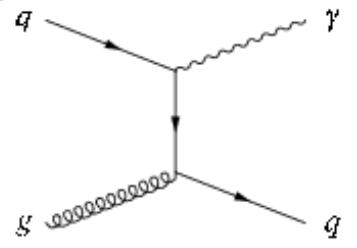
\includegraphics[width=0.4\textwidth]{gamma_jet}\\[1cm]
  \caption{Feynman diagram of a quark-gluon interaction, giving in output a high-energy quark and a prompt photon.}
  \label{gamma_jet}
\end{figure}

This report describes the analysis of \textgamma+jet events, in the first section will be described the CMS detector and
the hadronic jets. Then will be introduced the data that has been used for the analysis part.
For the analysis part will be implemented a multivariate analysis for photon identification this will be used for
measuring the \textgamma+jet purity in the data.

%%% Local Variables: 
%%% mode: latex
%%% TeX-master: "isae-report-template"
%%% End: 
